\section{Motivation} %1.1

The motivation for this project includes attention to one of the most serious environmental risks on the planet in the early 21st century, the accelerating global temperature.


According to the paper from Nature, climate change happened in the past 70 years \cite{parmesan2003globally}. It has already had effects on the environment around us. Glaciers are shrinking and ices are breaking up earlier on the lakes and rivers. 

\begin{figure}[!tbh]
\center
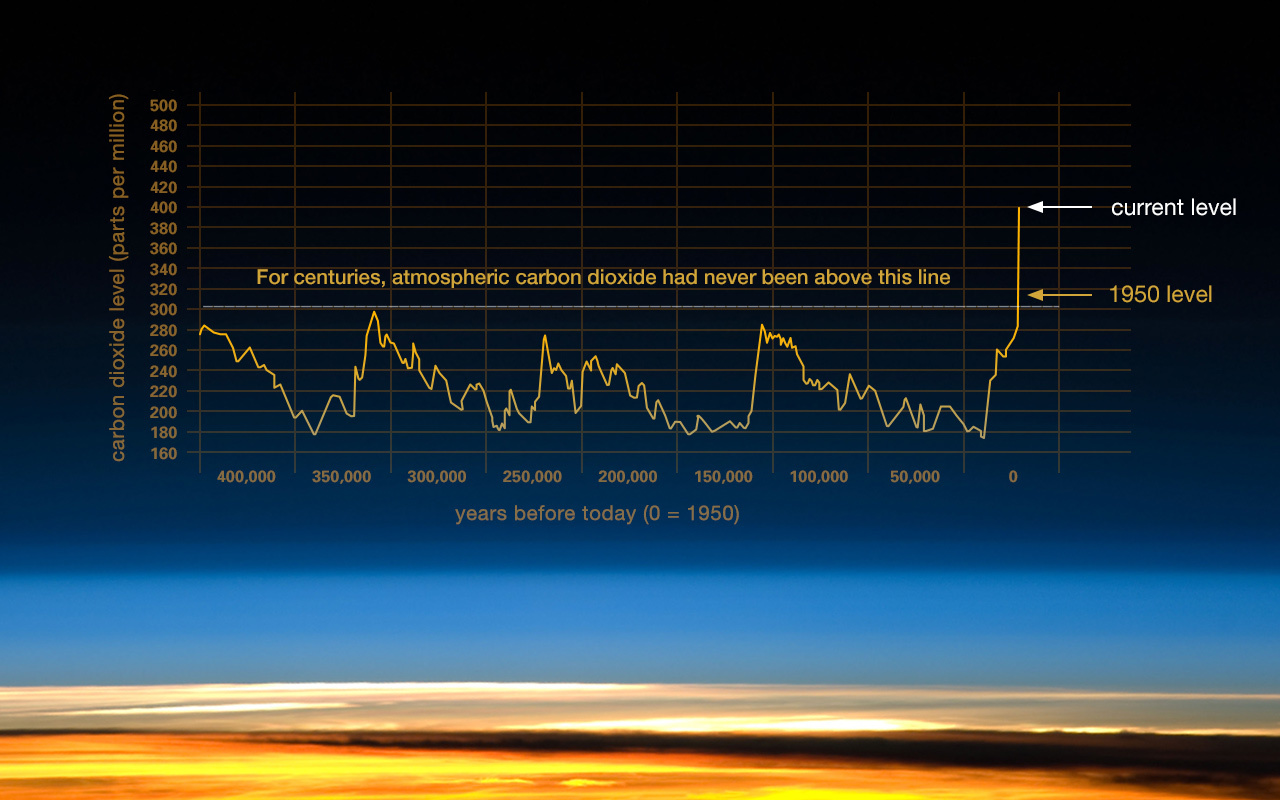
\includegraphics[scale=0.33]{Figure/1.1-NASA-CO2.jpeg}
\longcaption{The evidence that atmospheric CO2 has increased since the Industrial Revolution began}{\label{1.1-NASA-CO2} The evidence that atmospheric CO2 has increased since the Industrial Revolution began. Image courtesy: https://climate.nasa.gov/evidence}
\end{figure}

The greenhouse effect has been working since the formation of the earth. Without the greenhouse effect, the surface of the earth would be extremely cold, the temperature would drop to minus 20°C, the ocean would freeze, and life would not form. Most climate scientists agree that it is the human expansion that causes global warming \cite{epic337530}. As we know, carbon dioxide (CO2) is a significant component of the atmosphere. Atmospheric CO2 concentration has been increased by more than a third since the Industrial Revolution began \cite{epic337530}. More importantly, as shown in Figure \ref{1.1-NASA-CO2}, atmospheric carbon dioxide has exceeded the highest level in the past 400,000 years.

Therefore, what we are facing is not the issue of whether there is a greenhouse effect, but the issue that humans emit a large number of greenhouse gases into the atmosphere through the burning of fossil fuels, causing the drastic greenhouse effect and the earth’s climate.

When the world's average temperature rises by 1°C, huge changes will occur: sea levels will rise, mountain glaciers will retreat, and snow-covered areas will shrink. As the global temperature rises, it will lead to uneven precipitation. In some areas, precipitation increases, while in others, precipitation decreases. For example, the Sahel region in West Africa has been severely arid since 1965, while in North China, precipitation has been decreasing year after year since 1965. Compared with the 1950s, precipitation in North China has been reduced by 1/3, and water resources have been reduced by 1/2. China's annual drought-affected area is about 400 million acres. In normal years, the national irrigation area lacks 30 billion cubic meters of water each year, and the cities lack 6 billion cubic meters of water. 

When the average temperature of the world rises by 3°C, the world will suffer from food shortages. Due to rising temperatures, the global sea level has been rising at a rate of 1 to 2 millimetres per year in the past 100 years. It is expected that the sea level will continue to rise by 30 to 50 centimetres by 2050, which will flood a large amount of low-lying coastal land. Besides, due to climate changes have led to the aggravation of climatic disasters such as droughts, floods, and low temperatures, causing economic losses of more than tens of billions of dollars worldwide each year.


In this report, our team focuses on sea ice in the Arctic. We will look for the factors that we think affect the changes in Arctic sea ice, analyse their influence on the changes in sea ice, and select the two factors that we think are the most important. We will put these two influencing factors into our special situation model, and analyse the impact of significantly changing them on Arctic future sea ice.